\documentclass[tikz,border=10pt]{standalone}
\usepackage{tikz}
\usetikzlibrary{positioning}
\usetikzlibrary {arrows.meta}
\usepackage{tikz-feynman}
\begin{document}

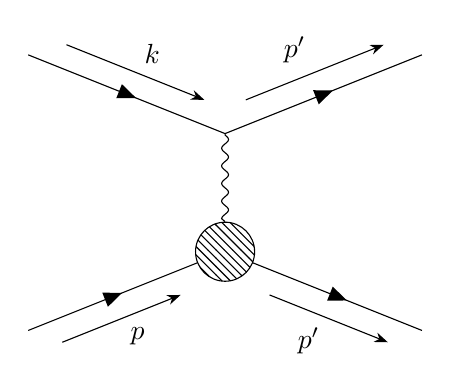
\begin{tikzpicture}
    \begin{feynman}
        %% fig j
        \vertex (j5) at (0,0);
        \vertex[above =-1.5cm  of j5, blob,anchor=center] (j6){};
        \vertex[above right =1cm  and 2.5cm of j5] (j3);
        \vertex[above right =1cm  and -2.5cm of j5] (j4);
        \vertex[above right =-1cm  and -2.5cm of j6] (j1);
        \vertex[above right =-1cm  and 2.5cm of j6] (j2);
        % \vertex[above right =-1.6cm  and -2.0cm of j6] (j1d);
        % \vertex[above right =-1.6cm  and 2.0cm of j6] (j2d);
        % 对各个顶点连线
        \diagram*{
        { [edge= fermion]
        (j1) --[momentum'=\(p\)] (j6)--[momentum'=\(p^\prime\)](j2),
        (j4) --[momentum=\(k\)] (j5)--[momentum=\(p^\prime\)](j3),
        },
        (j5)--[photon](j6);
        % (j1d)--[fermion,edge label'=\(t\)](j2d);
        };
    \end{feynman}
\end{tikzpicture}
\end{document}